% =====================================================================
%  Hard versus fuzzy eye-tracking gating of EEG windows: a controlled simulation study
%  ALL EXPERIMENTAL RESULTS IN THIS MANUSCRIPT ARE OBTAINED ON SYNTHETIC DATA.
%  Tables/figures in generated/ are produced by gfer/analyze_sim.py and gfer/analyze_noise.py.
% =====================================================================
\documentclass[11pt,a4paper]{article}
\usepackage[T1]{fontenc}
\usepackage[utf8]{inputenc}
\usepackage{lmodern}
\usepackage[margin=2.3cm]{geometry}
\usepackage{amsmath,amssymb,bm}
\usepackage{graphicx}
\usepackage{booktabs,multirow,tabularx,array}
\usepackage{xcolor}
\usepackage{algorithm}
\usepackage{algpseudocode}
\usepackage{tikz}
\usetikzlibrary{positioning,arrows.meta,fit,backgrounds,calc}
\usepackage[hidelinks]{hyperref}
\usepackage{caption}
\usepackage{framed}
\captionsetup{font=small,labelfont=bf,labelsep=space}
\newcommand{\pending}[1]{\textcolor{red!75!black}{\textbf{[#1]}}}
\newcommand{\simnote}{\textsuperscript{$\ast$}}

\title{Hard versus Fuzzy Eye-Tracking Gating of EEG Windows in a Sugeno Fuzzy Rule-Mining Emotion Recognizer: A Controlled Simulation Study}
\author{\pending{Author names and affiliations}}
\date{}

\begin{document}
\maketitle

% =====================================================================
\begin{abstract}
\noindent
Multimodal emotion recognition from electroencephalography (EEG) usually assumes that a stimulus label holds throughout the stimulus, although emotional responses are intermittent. A recent method addresses this by using an eye-tracking feature as a hard gate that retains only EEG segments at which the feature is high; the retained segments are described by wavelet-band entropy features and classified with genetic-algorithm-tuned Sugeno fuzzy rules. This paper asks whether replacing the crisp gate with a fuzzy gate, in which Low, Medium and High memberships of the normalised eye-tracking feature are mapped by a zero-order Sugeno rule base to a continuous window weight, is a better way to use the eye-tracking evidence. The weights enter feature selection, rule mining, genetic-algorithm fitness and trial-level aggregation, while all other components are unchanged. Because the true affective relevance of an EEG window cannot be observed in real recordings, the comparison is carried out in a controlled simulation: two synthetic 62-channel EEG and eye-tracking datasets (5 subjects, 60 one-minute trials, four classes each) with known emotional episodes, evaluated with trial-disjoint and leave-one-subject-out cross-validation over three seeds and five wavelet bands. \textbf{All results are obtained on synthetic data and are not estimates of real-world EEG performance.} When the gate feature tracked the episodes (pupil diameter, AUC 0.99), gating raised mean trial accuracy from 35.8\% to 55.2\% (hard) and 54.9\% (fuzzy) on the harder dataset and from 49.1\% to 66.0\% and 65.7\% on the easier one ($p\leq0.005$ against no gate). With the pupil gate, the fuzzy and hard gates did not differ significantly under either protocol ($p>0.4$), the fuzzy gate did not outperform a simple linear soft gate, and under increasing gate-signal noise the fuzzy gate did not degrade more gracefully than the hard gate. When the gate feature was chosen by minimum-redundancy-maximum-relevance ranking, as in the original method, fixation features were selected that carried little episode information (AUC 0.57) and neither gate helped consistently. Within this simulation, the form of the gate matters far less than whether the gating signal identifies the relevant windows.
\end{abstract}

\noindent\textbf{Keywords} Electroencephalogram (EEG) $\cdot$ Eye tracking $\cdot$ Emotion recognition $\cdot$ Fuzzy gating $\cdot$ Sugeno fuzzy inference system $\cdot$ Simulation study

\begin{framed}
\noindent\small\textbf{Data notice.} Every experimental number, table and figure in Sect.~\ref{sec:results} reports results on \emph{synthetic} EEG and eye-tracking data generated by the procedure in Sect.~\ref{sec:data}. Results marked \simnote{} are simulation results. They characterise the behaviour of the gating mechanisms under known ground truth and must not be compared with accuracies reported on real EEG corpora.
\end{framed}

% =====================================================================
\section{Introduction}
\label{sec:intro}

Automatic recognition of human affective states supports applications in mental-health assessment, adaptive human--computer interaction and user-experience evaluation. Among the physiological signals used for this purpose, the electroencephalogram (EEG) is attractive because it records cortical activity non-invasively with millisecond temporal resolution and at a cost far below that of functional neuroimaging \cite{Alarcao2019,Jenke2014}. EEG-based emotion recognition has progressed from band-power features with conventional classifiers to entropy-based and deep representations, and accuracies above 80\% are routinely reported on benchmark corpora such as DEAP, MAHNOB-HCI and the SEED family \cite{Koelstra2012,Soleymani2012db,ZhengLu2015,Zheng2019}.

Eye tracking provides a complementary, low-cost view of the same affective process. Pupil diameter increases with emotional arousal irrespective of valence \cite{Bradley2008,Partala2003}, and fixation and saccade statistics reflect the allocation of attention to a stimulus \cite{Lim2020}. Fusing EEG with eye-movement features improves recognition over either modality alone, for example from 78.51\% (EEG) and 77.80\% (eye movements) to 87.59\% with fuzzy-integral decision fusion \cite{Lu2015}, and to 85.11\% for four emotions on SEED-IV with multimodal deep learning \cite{Zheng2019}.

A less frequently addressed problem is the \emph{temporal validity of labels}. Emotion corpora assign one label to an entire stimulus, yet there is no guarantee that the intended emotion is present throughout the stimulus or that it is elicited at a predictable moment. When a long recording is cut into short windows that all inherit the stimulus label, many windows carry little affective information. Farhadi Sedehi et al.\ \cite{FarhadiSedehi2024a} proposed to use eye tracking as a \emph{gate} for this purpose: eight eye-tracking features are ranked with minimum-redundancy-maximum-relevance (mRMR) selection, the top-ranked feature (mean vertical pupil diameter on their data) is compared with a threshold, and only EEG segments at the corresponding moments are analysed with discrete wavelet transform (DWT) band entropies, mRMR feature selection and a Sugeno fuzzy inference system (S-FIS) whose rules are refined by a genetic algorithm (GA). They reported 94.42\% and 85.20\% alpha-band accuracy on SEED-IV and MAHNOB-HCI \cite{FarhadiSedehi2024a}, and later reused pupil-based gating in a Granger-causality model \cite{FarhadiSedehi2024b}.

The hard-threshold form of the gate has properties that motivate investigation. A window marginally below the threshold is discarded while one marginally above is retained with full weight, so small measurement fluctuations change the evidence used for training and testing. Pupil diameter is dominated by the light reflex and modulated by cognitive load, gaze position and tracking quality \cite{Mathot2018,Raiturkar2016,Holmqvist2012}, so treating a threshold crossing as a certain indicator of affective relevance ignores substantial uncertainty. Fuzzy set theory \cite{Zadeh1965} offers a natural way to express graded relevance, soft gating has a long history in machine learning \cite{Jacobs1991,Arevalo2020}, and fuzzy memberships have been used to weight training samples \cite{LinWang2002}. To the best of our knowledge, however, fuzzy memberships of eye-tracking features have not been used to weight EEG windows for emotion recognition.

Evaluating such a gate on real data faces a basic obstacle: the ground-truth affective relevance of each EEG window is unobservable, so one cannot tell whether a gate retains the right windows or merely changes the classifier's input distribution. This paper therefore studies the question in a \emph{controlled simulation} in which emotional episodes are known by construction. The research question is: \emph{Within an otherwise unchanged S-FIS-GA pipeline, does a fuzzy eye-tracking gate that assigns each EEG window a continuous relevance weight provide better or more robust recognition than the hard-threshold gate?} This was posed as a hypothesis to be tested, not assumed.

\subsection{Motivation}
Graded relevance is, in principle, a more faithful representation of an uncertain ocular indicator than a crisp threshold; a fuzzy gate never leaves a trial without evidence; and, because the classifier is itself a fuzzy rule base, a fuzzy gate keeps the whole pipeline interpretable. Whether these properties translate into accuracy or robustness is an empirical question that a simulation with known ground truth can answer cleanly before costly real-data studies.

\subsection{Contributions}
\begin{enumerate}
  \item We formalise the hard eye-tracking gate of \cite{FarhadiSedehi2024a} as a crisp window-weighting function and propose a fuzzy gate (M1) based on a Low/Medium/High partition and a zero-order Sugeno rule base, of which the hard gate (M0) is a limiting case.
  \item We integrate the window weights consistently into weighted mRMR selection, weighted entropy discretisation, weighted look-up-table rule mining, weighted GA fitness and weighted trial-level aggregation, so that M0 and M1 differ only in the gate.
  \item We compare M0, M1, a no-gate reference and a non-fuzzy linear soft gate on two synthetic datasets with known episodes, under trial-disjoint and leave-one-subject-out cross-validation, with paired statistical tests, a gate-noise robustness sweep and a direct measurement of how well each gate locates the episodes.
  \item We find\simnote{} that fuzzy and hard gating perform equivalently within the precision of the experiment, that the fuzzy gate is not more robust to gate noise, and that the choice of gating \emph{signal} dominates the choice of gating \emph{function}; in particular, label-driven mRMR selection of the gate feature can select features that do not indicate affective relevance.
\end{enumerate}

\subsection{Organization of the paper}
Section~\ref{sec:related} reviews related work and Sect.~\ref{sec:gap} states the research gap. Section~\ref{sec:method} describes the two gating models and the shared pipeline. Section~\ref{sec:data} describes the simulation design and Sect.~\ref{sec:setup} the experimental protocol. Section~\ref{sec:results} presents and discusses the results, Sect.~\ref{sec:limits} the limitations, and Sect.~\ref{sec:conclusion} concludes. Table~\ref{tab:abbr} lists the abbreviations.

\begin{table}[t]
\centering\small
\caption{List of abbreviations}\label{tab:abbr}
\begin{tabular}{@{}ll@{\hspace{2em}}ll@{}}
\toprule
Abbreviation & Description & Abbreviation & Description\\
\midrule
EEG & Electroencephalogram & mRMR & Min.-redundancy max.-relevance\\
ET & Eye tracking & S-FIS & Sugeno fuzzy inference system\\
DWT & Discrete wavelet transform & GA & Genetic algorithm\\
SampEn & Sample entropy & MF & Membership function\\
PermEn & Permutation entropy & LOSO & Leave-one-subject-out\\
SymbEn & Symbolic dynamics entropy & CV & Cross-validation\\
PhEn & Phase entropy & AUC & Area under the ROC curve\\
M0 & Hard-gated baseline & M1 & Proposed fuzzy-gated model\\
A1 & No-gate reference & A4 & Linear soft-gate ablation\\
SIM-H / SIM-E & Synthetic datasets (harder / easier) & pp & Percentage points\\
\bottomrule
\end{tabular}
\end{table}

% =====================================================================
\section{Related works}
\label{sec:related}

\subsection{EEG-based emotion recognition}
EEG emotion recognition pipelines typically consist of artefact removal, segmentation, feature extraction, feature selection and classification \cite{Alarcao2019}. Frequency-domain features remain dominant. Duan et al.\ \cite{Duan2013} introduced differential entropy (DE) and reported 84.22\% accuracy against 76.56\% for the energy spectrum, and Zheng and Lu \cite{ZhengLu2015} used deep belief networks on DE features of the SEED dataset to identify critical frequency bands and channels, obtaining 86.08\% average accuracy with comparable performance from reduced 4--12 channel montages. Time--frequency decomposition with the DWT is a common alternative to Fourier analysis because it provides band-limited sub-signals with good temporal localisation; Murugappan et al.\ \cite{Murugappan2010} used Daubechies-4 wavelets to extract alpha, beta and gamma components and reached 83.26\% with a k-nearest-neighbour classifier on five discrete emotions. Nonlinear complexity measures such as sample entropy \cite{Richman2000}, permutation entropy \cite{Bandt2002}, symbolic dynamics entropy \cite{Zebrowski2000} and phase entropy \cite{Rohila2019} have been adopted because EEG is non-stationary and nonlinear. Jenke et al.\ \cite{Jenke2014} compared features from 33 studies and found that such advanced features outperformed plain band power and that multivariate feature selection performed slightly better than univariate selection. The mRMR criterion \cite{Peng2005} is a widely used multivariate filter that selects features with high mutual information with the class and low mutual information with one another.

A recurring concern in this literature is evaluation validity. Li et al.\ \cite{Li2021} demonstrated that block-designed EEG experiments, in which training and test samples originate from the same continuous recording block, allow classifiers to exploit temporal correlations unrelated to the stimulus class. For emotion recognition, a review of 101 DEAP studies reported that segmentation leakage, feature selection on the full dataset and related errors were common and could inflate accuracy substantially \cite{Khan2025}, and a review of 216 papers reported inconsistent splitting and metrics across the field \cite{Kukhilava2025}. Both reviews are preprints and are cited here as indicative evidence. The cross-session drop reported for SEED-IV, from 85.11\% within sessions to 72.39\% across sessions \cite{Zheng2019}, further illustrates how strongly the evaluation protocol affects reported performance.

\subsection{Eye tracking and emotion}
The pupil dilates in response to emotionally arousing pictures and sounds, both pleasant and unpleasant, and this dilation co-varies with skin conductance, indicating sympathetic activation \cite{Bradley2008,Partala2003}. Pupil size therefore indexes arousal rather than valence. It is also governed primarily by the light and near responses, of which the psychosensory component is comparatively small \cite{Mathot2018}. For dynamic stimuli such as films, luminance changes must be modelled or removed before pupil size can be interpreted as arousal \cite{Raiturkar2016}, and Lu et al.\ explicitly removed the light reflex before using pupil features for emotion recognition \cite{Lu2015}. Pupil and gaze data further suffer from blinks, data loss and limited precision, which must be measured and reported \cite{Holmqvist2012}; standard preprocessing guidelines address blink removal, interpolation and smoothing \cite{Kret2019}. Lim et al.\ \cite{Lim2020} surveyed eye-tracking emotion recognition and identified pupil diameter, fixation, saccade and blink features as the most commonly used, while noting that eye tracking alone remains a relatively immature approach.

\subsection{Multimodal EEG and eye-tracking emotion recognition}
Zheng et al.\ \cite{ZhengDong2014} combined EEG with pupil-diameter features from five subjects watching film clips and obtained 71.77\% (EEG), 58.90\% (eye tracking) and 73.59\% (feature-level fusion) for three classes. Soleymani et al.\ \cite{Soleymani2012mm} fused EEG with pupil response and gaze distance at decision level and, under a participant-independent protocol, reached 68.5\% and 76.4\% for three-class valence and arousal, respectively. Lu et al.\ \cite{Lu2015} compared feature-level, decision-level and fuzzy-integral fusion of 16 eye-movement features with EEG; the fuzzy integral, which combines classifier outputs according to the importance of each source \cite{ChoKim1995}, produced the best accuracy of 87.59\%. EmotionMeter \cite{Zheng2019} introduced the four-class SEED-IV dataset and showed that EEG and eye movements are complementary: EEG recognised happiness better, whereas eye movements recognised fear better. Liu et al.\ \cite{Liu2022} compared deep canonical correlation analysis and bimodal autoencoders across five datasets, adding weighted-sum and attention-based fusion, and achieved 87.5\% on SEED-IV. Fu et al.\ \cite{Fu2023} aligned 4-s EEG and eye-movement windows in a two-branch network with multi-scale attention fusion and reported 87.32\% on SEED-IV.

In all of these studies the eye-tracking signal is a source of \emph{features} or \emph{decisions} to be fused with EEG. The gated approach of Farhadi Sedehi et al.\ \cite{FarhadiSedehi2024a,FarhadiSedehi2024b} is different in kind: eye tracking determines \emph{which EEG segments} are analysed, so it acts as a temporal selector rather than as a feature source. Table~\ref{tab:related} summarises the reviewed multimodal studies. Accuracies are copied from the original papers and are not directly comparable, because datasets, class definitions and validation protocols differ.

\begin{table}[t]
\centering\scriptsize
\caption{Summary of related EEG and eye-tracking emotion-recognition studies (results as reported by the original authors)}\label{tab:related}
\begin{tabularx}{\linewidth}{@{}p{0.9cm}p{1.5cm}p{3.0cm}p{2.0cm}p{1.6cm}X@{}}
\toprule
Ref. & Dataset & Method & Use of eye tracking & Result & Limitation\\
\midrule
\cite{ZhengDong2014} & Own (5 subj., 3 cl.) & PSD/DE, SVM, FLF/DLF & Pupil features fused & 73.59\% & Very small sample$^\dagger$\\
\cite{Soleymani2012mm} & MAHNOB proto. (24 subj.) & EEG + pupil/gaze, DLF & Features fused & 68.5\% V, 76.4\% A & Trial-level only; no temporal selection$^\ast$\\
\cite{Lu2015} & SEED-style (9 subj., 3 cl.) & DE + 16 eye features, fuzzy integral & Features + fuzzy DLF & 87.59\% & Within-session; fusion at output level$^\ast$\\
\cite{Zheng2019} & SEED-IV (4 cl.) & DE/PSD, multimodal DNN & Features fused & 85.11\% & Cross-session drop to 72.39\%\\
\cite{Liu2022} & SEED, SEED-IV, SEED-V, DEAP, DREAMER & DCCA/BDAE, attention fusion & Features fused & 87.5\% (SEED-IV) & Learned modality weights, not per window$^\ast$\\
\cite{Fu2023} & SEED-IV & Two-branch net, multi-scale attention & Features fused & 87.32\% & Black-box; weights not temporal$^\ast$\\
\cite{FarhadiSedehi2024a} & SEED-IV, MAHNOB-HCI (4 cl.) & DWT entropies, mRMR, S-FIS-GA & Hard pupil gate selects EEG segments & 94.42\%, 85.20\% & Segment-level 5-fold CV; crisp gate$^\ast$\\
\cite{FarhadiSedehi2024b} & MAHNOB-HCI (2 cl.) & Granger causality images, ResNet-18 & Hard pupil gate & 91.00\% & Crisp gate$^\ast$\\
\bottomrule
\multicolumn{6}{@{}l}{\scriptsize $^\dagger$ stated by the authors; $^\ast$ our analysis. FLF/DLF: feature-/decision-level fusion; V/A: valence/arousal.}
\end{tabularx}
\end{table}

\subsection{Fuzzy logic in emotion recognition and soft gating}
Fuzzy sets \cite{Zadeh1965} represent graded membership, and Takagi--Sugeno--Kang (TSK) models \cite{TakagiSugeno1985} combine fuzzy antecedents with functional or constant consequents. Rules can be generated from data with table look-up schemes such as that of Wang and Mendel \cite{WangMendel1992}, which is close to the look-up-table rule extraction used in the baseline, and membership parameters can be learned with neuro-fuzzy systems such as ANFIS \cite{Jang1993}. In emotion recognition, fuzzy rules have been used as interpretable EEG classifiers \cite{Matiko2014,FarhadiSedehi2024a}, fuzzy linguistic summaries have been applied to EEG time series \cite{Kaya2024}, and fuzzy integrals have fused EEG and eye-movement classifiers \cite{Lu2015,ChoKim1995}.

Gating, the use of one signal to modulate the contribution of another, has been studied separately. The mixture-of-experts model \cite{Jacobs1991} uses a soft gating network to weight expert outputs, and gated multimodal units learn multiplicative gates that decide how much each modality contributes \cite{Arevalo2020}. Classical classifier-combination theory analyses weighted sum and product rules \cite{Kittler1998}, and quality-aware fusion incorporates measured signal quality into score combination \cite{Nandakumar2008}. Fuzzy support vector machines assign each training sample a fuzzy membership that scales its influence on learning, reducing the effect of noisy samples \cite{LinWang2002}. These works establish soft weighting as an alternative to hard selection, but their weights are either learned and opaque, applied to modalities rather than time windows, or derived from the training sample itself rather than from a second modality.

% =====================================================================

% =====================================================================
\section{Research gap and contributions}
\label{sec:gap}

The literature leads to four observations. (a) EEG and eye-tracking fusion consistently improves on single modalities \cite{Lu2015,Zheng2019,Liu2022}, but eye tracking is almost always used as a feature source rather than as an indicator of \emph{when} EEG carries affective information. (b) The only approach we found that uses eye tracking for temporal selection of EEG \cite{FarhadiSedehi2024a,FarhadiSedehi2024b} applies a crisp threshold to a single pupil feature. (c) The ocular signal used for gating is uncertain: it reflects arousal rather than a specific emotion, is confounded by luminance, cognitive load and gaze geometry, and contains missing and noisy samples \cite{Bradley2008,Mathot2018,Raiturkar2016,Holmqvist2012}. (d) Fuzzy soft weighting exists in related forms \cite{LinWang2002,Jacobs1991,Lu2015}, but our search found no study that maps eye-tracking memberships to continuous relevance weights for EEG windows.

Observations (b) and (c) are our analysis; the original authors acknowledge the limited input capacity of the S-FIS and the scarcity of multimodal databases \cite{FarhadiSedehi2024a}, not the brittleness of the threshold. A further gap is methodological: published evaluations of gating report only end-to-end accuracy on real data, where the relevance of each window is unknown, and use segment-level random cross-validation, in which windows from the same trial fall into both training and test sets \cite{FarhadiSedehi2024a,Li2021,Khan2025}. Neither allows the effect of the gate to be separated from other factors. This paper addresses that gap with a simulation in which relevance is known and with trial- and subject-disjoint evaluation. Combining EEG, eye tracking and fuzzy logic is not novel in itself \cite{Lu2015,FarhadiSedehi2024a}; the specific question studied is the \emph{form of the eye-tracking gate}, with all other components fixed. Our literature search was not a formal systematic review, so the novelty claim is stated to the best of our knowledge.

% =====================================================================
\section{Methodology}
\label{sec:method}

\subsection{Overall architecture}
Figure~\ref{fig:arch} shows the architecture shared by all compared configurations. The EEG branch (preprocessing, windowing, DWT band decomposition, entropy features, mRMR selection and S-FIS-GA classification) and the eye-tracking feature branch are identical; configurations differ only in the gate, which converts the gating feature of each window into a weight $w_k$. Table~\ref{tab:notation} lists the notation. The implementation follows the description in \cite{FarhadiSedehi2024a}; where that description is incomplete, the choice made is stated explicitly.

\begin{figure}[t]
\centering
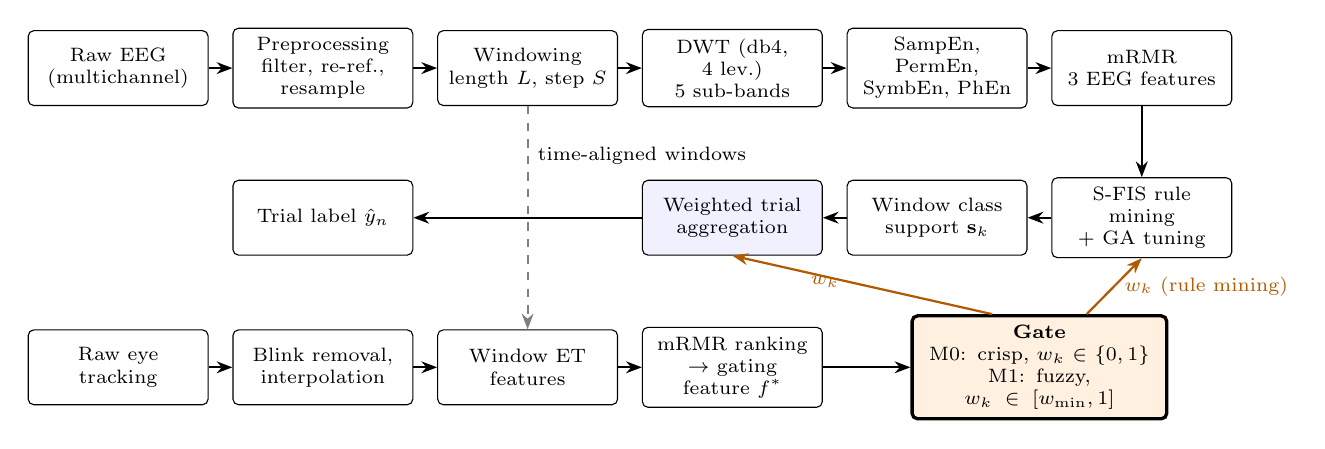
\begin{tikzpicture}[
  font=\scriptsize,
  box/.style={draw, rounded corners=2pt, align=center, minimum height=0.95cm, text width=2.05cm, fill=white},
  gate/.style={draw, very thick, rounded corners=2pt, align=center, minimum height=1.25cm, text width=3.0cm, fill=orange!12},
  arr/.style={-{Stealth[length=2mm]}, thick},
  warr/.style={-{Stealth[length=2mm]}, thick, orange!70!black}]
\def\dx{2.6}
% row 1: EEG feature chain
\node[box] (eeg) at (0,0) {Raw EEG\\(multichannel)};
\node[box] (pre) at (\dx,0) {Preprocessing\\filter, re-ref., resample};
\node[box] (win) at (2*\dx,0) {Windowing\\length $L$, step $S$};
\node[box] (dwt) at (3*\dx,0) {DWT (db4, 4 lev.)\\5 sub-bands};
\node[box] (ent) at (4*\dx,0) {SampEn, PermEn,\\SymbEn, PhEn};
\node[box] (mrmr) at (5*\dx,0) {mRMR\\3 EEG features};
% row 2: classification and aggregation
\node[box] (fis) at (5*\dx,-1.9) {S-FIS rule mining\\+ GA tuning};
\node[box] (sup) at (4*\dx,-1.9) {Window class\\support $\mathbf{s}_k$};
\node[box, fill=blue!6] (agg) at (3*\dx,-1.9) {Weighted trial\\aggregation};
\node[box] (out) at (1*\dx,-1.9) {Trial label $\hat{y}_n$};
% row 3: eye-tracking chain
\node[box] (et) at (0,-3.8) {Raw eye\\tracking};
\node[box] (etp) at (\dx,-3.8) {Blink removal,\\interpolation};
\node[box] (etf) at (2*\dx,-3.8) {Window ET\\features};
\node[box] (etm) at (3*\dx,-3.8) {mRMR ranking\\$\rightarrow$ gating feature $f^\ast$};
\node[gate] (g) at (4.5*\dx,-3.8) {\textbf{Gate}\\M0: crisp, $w_k\in\{0,1\}$\\M1: fuzzy, $w_k\in[w_{\min},1]$};
% arrows
\draw[arr] (eeg)--(pre); \draw[arr] (pre)--(win); \draw[arr] (win)--(dwt); \draw[arr] (dwt)--(ent); \draw[arr] (ent)--(mrmr);
\draw[arr] (mrmr)--(fis); \draw[arr] (fis)--(sup); \draw[arr] (sup)--(agg); \draw[arr] (agg)--(out);
\draw[arr] (et)--(etp); \draw[arr] (etp)--(etf); \draw[arr] (etf)--(etm); \draw[arr] (etm)--(g);
\draw[arr, dashed, gray] (win.south) -- node[pos=0.22, right, text=black]{time-aligned windows} (etf.north);
\draw[warr] ($(g.north)+(0.6,0)$) -- node[right]{$w_k$ (rule mining)} (fis.south);
\draw[warr] ($(g.north)+(-0.6,0)$) -- node[left, pos=0.55]{$w_k$} (agg.south);
\end{tikzpicture}
\caption{Common architecture of the baseline (M0) and the proposed model (M1). All blocks are shared except the gate (shaded), which produces the window weight $w_k$ used in feature selection, rule mining, GA fitness and trial-level aggregation.}
\label{fig:arch}
\end{figure}

\begin{table}[t]
\centering\small
\caption{Key notations}\label{tab:notation}
\begin{tabular}{@{}ll@{}}
\toprule
Notation & Description\\
\midrule
$n$, $k$, $K_n$ & Trial index; window index; number of windows in trial $n$ ($K_n=15$)\\
$\mathbf{x}_{n,k}\in\mathbb{R}^{3}$ & Selected EEG entropy features of window $k$ (S-FIS inputs)\\
$z_{n,k}$, $\tilde z_{n,k}$ & Raw and normalised gating feature of window $k$\\
$\mu_{L},\mu_{M},\mu_{H}$ & Low/Medium/High membership functions of the fuzzy gate\\
$r_{L},r_{M},r_{H}$ & Constant consequents (relevance levels) of the gate rules\\
$w_{n,k}$ & Window weight: $\{0,1\}$ for M0, $[r_L,1]$ for M1\\
$\alpha_j(\mathbf{x})$, $\mathrm{CF}_j$ & Firing strength and certainty factor of classification rule $j$\\
$p_{n,k,c}$, $S_{n,c}$ & Window class score; aggregated trial score for class $c$\\
$C$ & Number of classes ($C=4$)\\
\bottomrule
\end{tabular}
\end{table}

\subsection{Shared EEG pipeline}
\paragraph{Preprocessing and windowing.} EEG is band-pass filtered (fourth-order zero-phase Butterworth, 1--60~Hz), notch-filtered at 50~Hz ($Q=30$) and resampled to 128~Hz, following \cite{FarhadiSedehi2024a}. Each 60-s trial is divided into $K_n=15$ non-overlapping 4-s windows.

\paragraph{Band decomposition.} A four-level DWT with the Daubechies-4 wavelet \cite{Mallat1989} yields, at 128~Hz, the sub-bands A4 (0--4~Hz, delta), D4 (4--8~Hz, theta), D3 (8--16~Hz, alpha), D2 (16--32~Hz, beta) and D1 (32--64~Hz, gamma). These dyadic boundaries only approximate the conventional bands quoted in \cite{FarhadiSedehi2024a}. Each sub-band is reconstructed to full length before windowing, so entropies are computed on 512-sample signals rather than on decimated coefficient vectors, which would be too short for embedding dimension 5.

\paragraph{Entropy features.} For each channel, sub-band and window, four entropies are computed with the parameters of \cite{FarhadiSedehi2024a}: sample entropy \cite{Richman2000}
\begin{equation}
\mathrm{SampEn}(m,r) = -\ln\frac{A}{B},
\end{equation}
where $B$ and $A$ count template pairs of length $m$ and $m+1$ within tolerance $r$ (self-matches excluded), with $m=5$, delay 2 and $r=0.15\,\sigma$; permutation entropy \cite{Bandt2002}
\begin{equation}
\mathrm{PermEn} = -\sum_{i=1}^{m!} p_i \ln p_i,
\end{equation}
with order $m=5$ and delay 2; symbolic dynamics entropy \cite{Zebrowski2000} with word length 5, delay 2 and alphabet size 3; and phase entropy \cite{Rohila2019}
\begin{equation}
\mathrm{PhEn} = -\sum_{i=1}^{k} p(i)\log p(i)
\end{equation}
over $k=5$ sectors of the second-order difference plot. With 62 channels, each window yields $4\times62=248$ features per band. Features are z-scored per subject, which uses no labels.

\paragraph{Weighted feature selection.} Three features per band are selected with the mRMR criterion \cite{Peng2005}
\begin{equation}
f_{t+1} = \arg\max_{f_j\notin\mathcal{S}_t}\Big[I_w(f_j;y) - \frac{1}{|\mathcal{S}_t|}\sum_{f_i\in\mathcal{S}_t} I_w(f_j;f_i)\Big],
\label{eq:mrmr}
\end{equation}
where $I_w$ is the mutual information of features discretised into 10 quantile bins, computed from a contingency table in which each training window contributes its weight $w_{n,k}$. For binary weights this is ordinary mRMR on the retained windows.

\paragraph{Sugeno fuzzy classifier.} Each selected feature is partitioned into three levels (Low, Medium, High) by greedy entropy-based discretisation of the (weighted) training data, and triangular membership functions with shoulders are centred on the resulting intervals \cite{FarhadiSedehi2024a}. Candidate rules
\begin{equation}
R_j:\ \text{IF } x_1 \text{ is } A_{j1} \text{ AND } x_2 \text{ is } A_{j2} \text{ AND } x_3 \text{ is } A_{j3} \text{ THEN class} = c_j \text{ with } \mathrm{CF}_j
\end{equation}
are generated by the look-up-table method \cite{WangMendel1992}: each training window proposes the antecedent formed by its maximum-membership levels with degree $w_{n,k}\prod_i\max_\ell\mu_{i\ell}(x_i)$, and conflicting rules keep the class with the largest summed degree. The firing strength uses the product t-norm, $\alpha_j(\mathbf{x})=\prod_{i}\mu_{A_{ji}}(x_i)$, and the window class score is the zero-order Sugeno output with class-indicator consequents,
\begin{equation}
p_{n,k,c} = \frac{\sum_{j:\,c_j=c}\mathrm{CF}_j\,\alpha_j(\mathbf{x}_{n,k})}{\sum_{j}\mathrm{CF}_j\,\alpha_j(\mathbf{x}_{n,k})},
\label{eq:score}
\end{equation}
with the class prior used when no rule fires.

\paragraph{GA rule tuning.} The GA encodes, for every mined rule, an activity bit and its antecedent levels (including ``don't care''); consequents and certainty factors are recomputed from the weighted training data for each candidate (class of maximum weighted firing mass; certainty factor equal to confidence minus the mean confidence of the other classes). The population size is 27 \cite{FarhadiSedehi2024a}, with two elite individuals, tournament selection of size 3, rule-level uniform crossover (rate 0.8), activity and antecedent mutation (rate 0.05 each) and termination after 10 generations without improvement (maximum 500). The fitness combines accuracy and coverage as in \cite{FarhadiSedehi2024a}, both weighted by the window weights, with a small rule-count penalty:
\begin{equation}
\Phi = \mathrm{Acc}_w + 0.2\,\mathrm{Cov}_w - 0.01\,\frac{R_{\mathrm{active}}}{R},\quad
\mathrm{Acc}_w = \frac{\sum w_{n,k}\mathbf{1}[\hat y_{n,k}=y_n]}{\sum w_{n,k}},\quad
\mathrm{Cov}_w = \frac{\sum w_{n,k}\mathbf{1}[\exists j:\alpha_j>0]}{\sum w_{n,k}}.
\label{eq:fit}
\end{equation}

\paragraph{Weighted trial-level aggregation.} Window scores are combined into a trial prediction with the same weights,
\begin{equation}
S_{n,c} = \frac{\sum_{k=1}^{K_n} w_{n,k}\,p_{n,k,c}}{\sum_{k=1}^{K_n} w_{n,k}},\qquad \hat y_n = \arg\max_{c} S_{n,c},
\label{eq:agg}
\end{equation}
which is a weighted sum rule \cite{Kittler1998}. Every configuration therefore produces exactly one prediction for every trial, so all are evaluated on the same set of trials.

\subsection{Eye-tracking features and gating feature}
Eight features are computed per 4-s window as in \cite{FarhadiSedehi2024a}: mean, standard deviation and maximum of fixation duration, fixation frequency, and mean and standard deviation of pupil diameter in the horizontal and vertical directions; blink samples are excluded. Two ways of choosing the gating feature are studied. In \textbf{G-pupil}, the gate uses the mean vertical pupil diameter, the feature reported by \cite{FarhadiSedehi2024a}. In \textbf{G-mRMR}, the original selection procedure is reproduced: the eight features are z-scored per subject, ranked by mRMR against the class label on the training windows of each fold, and the top-ranked feature is used.

The gating feature is normalised within each trial with robust percentile scaling, which uses no labels:
\begin{equation}
\tilde z_{n,k} = \operatorname{clip}_{[0,1]}\left(\frac{z_{n,k}-P_{5}^{(n)}}{P_{95}^{(n)}-P_{5}^{(n)}}\right),
\label{eq:norm}
\end{equation}
where $P_{5}^{(n)}$ and $P_{95}^{(n)}$ are percentiles over the windows of trial $n$.

\subsection{Hard gate (M0)}
The original description uses ``the maximum'' of the gating feature as threshold without specifying its scope or how many windows are kept. Read literally, it would keep a single window per trial. Following the team's implementation, the threshold is the within-trial 60th percentile,
\begin{equation}
w^{\mathrm{M0}}_{n,k} = \mathbf{1}\big[\tilde z_{n,k} \geq Q_{0.6}^{(n)}(\tilde z)\big],
\label{eq:hard}
\end{equation}
which retains about 40\% of the windows of every trial; windows with $w=0$ are excluded from all training steps and from aggregation.

\subsection{Fuzzy gate (M1)}
\paragraph{Fuzzification.} The normalised feature is described by three fuzzy sets forming a Ruspini partition ($\mu_L+\mu_M+\mu_H=1$):
\begin{align}
\mu_{L}(\tilde z) &= \operatorname{clip}_{[0,1]}\!\Big(\frac{c-\tilde z}{c-a_1}\Big),\qquad
\mu_{H}(\tilde z) = \operatorname{clip}_{[0,1]}\!\Big(\frac{\tilde z-c}{b_2-c}\Big),\\
\mu_{M}(\tilde z) &= \max\!\Big(0,\min\!\Big(\frac{\tilde z-a_1}{c-a_1},\frac{b_2-\tilde z}{b_2-c}\Big)\Big),
\end{align}
with $a_1=0.2$, $c=0.5$ and $b_2=0.8$ (Fig.~\ref{fig:mf}a). These values were fixed a priori and not tuned.

\paragraph{Gate rule base and weight.} A zero-order Sugeno rule base maps memberships to relevance: IF $\tilde z$ is Low THEN relevance $=r_L$; IF $\tilde z$ is Medium THEN relevance $=r_M$; IF $\tilde z$ is High THEN relevance $=r_H$, with $(r_L,r_M,r_H)=(0.1,0.5,1)$. The weight is
\begin{equation}
w^{\mathrm{M1}}_{n,k} = \frac{\mu_L(\tilde z_{n,k})\,r_L + \mu_M(\tilde z_{n,k})\,r_M + \mu_H(\tilde z_{n,k})\,r_H}{\mu_L(\tilde z_{n,k})+\mu_M(\tilde z_{n,k})+\mu_H(\tilde z_{n,k})}\ \in [r_L,1],
\label{eq:fuzzy}
\end{equation}
so no window is discarded. If the Medium set shrinks to zero width at the threshold and $r_L\to0$, Eq.~\eqref{eq:fuzzy} reduces to a crisp step, so M0 is a limiting case of M1. With one input and a Ruspini partition, Eq.~\eqref{eq:fuzzy} is a monotone piecewise-linear function of $\tilde z$ (Fig.~\ref{fig:mf}b). To test whether the fuzzy formulation adds anything beyond softness, the linear soft gate $w^{\mathrm{A4}}_{n,k}=\max(r_L,\tilde z_{n,k})$ is included as an ablation.

\begin{figure}[t]
\centering
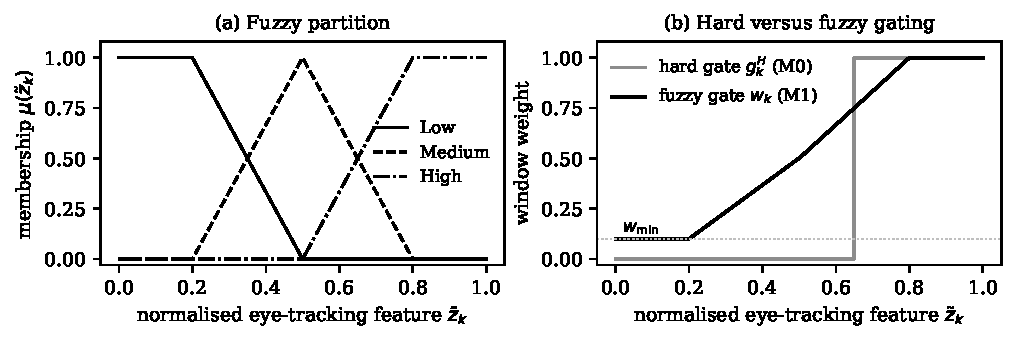
\includegraphics[width=0.95\linewidth]{figures/fuzzy_gate_mf.pdf}
\caption{(a) Fuzzy partition of the normalised gating feature. (b) Fuzzy gate weight (Eq.~\ref{eq:fuzzy}) compared with a hard gate. Parameters $a_1=0.2$, $c=0.5$, $b_2=0.8$, $r=(0.1,0.5,1)$; the hard-gate step is drawn at $\tau=0.65$ for illustration, whereas M0 places its threshold at the within-trial 60th percentile.}
\label{fig:mf}
\end{figure}

Algorithm~\ref{alg:m1} summarises one cross-validation fold, and Table~\ref{tab:m0m1} lists the components of every configuration.

\begin{algorithm}[t]
\caption{Gated S-FIS-GA recognition for one cross-validation fold}\label{alg:m1}
\small
\begin{algorithmic}[1]
\Require Training trials $\mathcal{T}$, test trials $\mathcal{V}$ (disjoint), gate type $\in\{$none, hard, fuzzy, linear$\}$
\Ensure Trial predictions $\{\hat y_n\}_{n\in\mathcal{V}}$
\State Compute 8 ET features and $5\times4\times62$ EEG entropies for every 4-s window
\State Choose gating feature (fixed pupil-Y, or mRMR rank on windows of $\mathcal{T}$)
\State Normalise it within each trial (Eq.~\ref{eq:norm}); compute $w_{n,k}$ (Eq.~\ref{eq:hard} or \ref{eq:fuzzy})
\For{each band}
  \State Select 3 EEG features by weighted mRMR on $\mathcal{T}$ (Eq.~\ref{eq:mrmr})
  \State Fit weighted entropy cut points and triangular MFs on $\mathcal{T}$
  \State Mine look-up-table rules with degrees scaled by $w_{n,k}$
  \State Tune the rule base with the GA using fitness $\Phi$ (Eq.~\ref{eq:fit})
  \For{each $n\in\mathcal{V}$} compute $p_{n,k,c}$ (Eq.~\ref{eq:score}) and $\hat y_n$ (Eq.~\ref{eq:agg}) \EndFor
\EndFor
\end{algorithmic}
\end{algorithm}

\begin{table}[t]
\centering\small
\caption{Components of the compared configurations; only the gate differs}\label{tab:m0m1}
\begin{tabular}{@{}lllll@{}}
\toprule
Component & A1 (no gate) & M0 (hard) & M1 (fuzzy) & A4 (linear)\\
\midrule
EEG pipeline, ET features & \multicolumn{4}{c}{shared (Sect.~4.2--4.3)}\\
Gating feature & -- & \multicolumn{3}{c}{G-pupil or G-mRMR (shared)}\\
Window weight & $1$ & Eq.~\eqref{eq:hard} & Eq.~\eqref{eq:fuzzy} & $\max(0.1,\tilde z)$\\
Effective share of training windows\simnote & 100\% & 41.8\% & 45.7\% & 44.3\%\\
Weights in mRMR, cuts, rule mining, GA & -- & \multicolumn{3}{c}{yes (Eqs.~\ref{eq:mrmr}, \ref{eq:fit})}\\
Trial aggregation & \multicolumn{4}{c}{Eq.~\eqref{eq:agg}}\\
\bottomrule
\end{tabular}
\end{table}

% =====================================================================
\section{Simulation design}
\label{sec:data}

Two synthetic datasets were generated with the procedure below (implementation in \texttt{gfer/demo.py}). They are designed so that every pipeline stage has something to find and, crucially, so that the windows carrying class information are known.

\paragraph{Structure.} Each dataset has 5 simulated subjects and 12 trials per subject (3 per class: sad, happy, fear, neutral), i.e.\ 60 trials of 60~s and 900 four-second windows. EEG has 62 channels in the SEED-IV montage at 200~Hz; eye tracking has 60~Hz pupil diameters in the horizontal and vertical directions and a fixation sequence.

\paragraph{Background EEG.} Eight pink-noise sources are mixed into the channels through a subject-specific random matrix, with posterior alpha activity, independent channel noise, 50~Hz line interference and channel DC offsets.

\paragraph{Emotional episodes.} Each trial contains three non-overlapping episodes of 6--10~s placed at random after the first 4~s (mean length 7.9~s in SIM-H and 8.1~s in SIM-E). On average 39.3\% (SIM-H) and 40.3\% (SIM-E) of windows overlap an episode by at least half their length. Class information exists in the EEG \emph{only} during episodes: a band-limited component with class-specific bandwidth, amplitude and burstiness (sad narrow-band and regular, happy medium bandwidth, fear broadband and bursty, neutral none) is added to T7, T8, Fp2 and neighbouring channels, with band strengths alpha $>$ beta $>$ gamma $>$ theta $>$ delta, and a subject-specific gain.

\paragraph{Eye-tracking signals.} During episodes the vertical pupil diameter dilates by a class-dependent amount (0.35--0.65~mm; the horizontal diameter by 60\% of this) with 1.5-s ramps, on top of a subject-specific baseline (3.0--4.2~mm) and a slow random drift. Two \emph{distractor} dilations of 3--5~s (0.25~mm) per trial carry no EEG change, so the pupil is an informative but imperfect indicator. About 15 blinks per trial are inserted as missing samples. Fixation durations are gamma-distributed around 260~ms and are multiplied by a class-dependent factor (sad 1.35, happy 1.10, fear 0.80, neutral 1.00) during episodes, so fixation features carry class information but only weak episode information.

\paragraph{Difficulty levels.} SIM-H (``harder'') uses class-signal strength 1.0 and generator seed 0; SIM-E (``easier'') uses strength 3.0 and seed 1. Both datasets were regenerated from these settings and verified to be identical to the files used in the experiments.

Table~\ref{tab:simdata} summarises the design. The simulation deliberately encodes the assumption that motivates gating, namely that affective information is intermittent and that pupil dilation co-occurs with it. The results therefore show how the gates behave when this assumption holds; they do not show that it holds in real recordings.

\begin{table}[t]
\centering\small
\caption{Synthetic datasets (generator \texttt{gfer/demo.py})}\label{tab:simdata}
\begin{tabular}{@{}lll@{}}
\toprule
Property & SIM-H & SIM-E\\
\midrule
Subjects / trials / windows & 5 / 60 / 900 & 5 / 60 / 900\\
Classes (trials per class) & sad, happy, fear, neutral (15 each) & same\\
EEG & 62 ch, 200 Hz, 60 s per trial & same\\
Eye tracking & pupil X/Y 60 Hz, fixations, blinks & same\\
Episodes per trial; windows in episode & 3; 39.3\% & 3; 40.3\%\\
Distractor pupil dilations per trial & 2 & 2\\
Class-signal strength; seed & 1.0; 0 & 3.0; 1\\
\bottomrule
\end{tabular}
\end{table}

% =====================================================================
\section{Experimental setup}
\label{sec:setup}

\paragraph{Configurations.} Four gates are compared: A1 (no gate), M0 (hard), M1 (fuzzy) and A4 (linear soft). Each is run with both gating-feature choices (G-pupil and G-mRMR), on both datasets, for all five bands, with three fuzzy levels per input.

\paragraph{Validation and leakage control.} Evaluation is at trial level. Two protocols are used: (P1) stratified trial-disjoint 5-fold CV, with 12 test trials per fold, and (P2) leave-one-subject-out (LOSO) CV over the 5 subjects. No trial (P1) or subject (P2) contributes windows to both training and test data. All label-dependent steps, namely gating-feature selection in G-mRMR, EEG mRMR, discretisation and the GA, are fitted on training trials only. The two label-free normalisations (per-subject z-scoring of entropies and per-trial scaling of the gating feature) are applied identically to every configuration. Each setting is repeated with three seeds, which change the P1 fold assignment and the GA's random operations, giving 15 (seed, band) results per configuration, dataset and protocol. M0, M1, A1 and A4 share folds and seeds.

\paragraph{Gate-noise robustness.} To test the claim that fuzzy gating tolerates an uncertain eye signal, Gaussian noise with standard deviation $\kappa\in\{0.5,1,2\}$ times the within-subject standard deviation of the pupil feature is added to the G-pupil gating feature before normalisation (protocol P1, all bands, three seeds).

\paragraph{Gate quality.} Because episodes are known, the gates are also assessed directly. For each window, the label ``in episode'' is compared with the normalised gating feature (AUC), with the hard gate's retained set (precision and recall) and with the soft gates' weights (weighted precision $\sum_k w_k e_k/\sum_k w_k$, where $e_k=1$ if window $k$ lies in an episode).

\paragraph{Metrics and statistics.} Accuracy, balanced accuracy and macro-averaged precision, recall and F1 are computed over the pooled trial predictions of all folds of a run. Because classes are balanced, balanced accuracy equals macro recall and chance accuracy is 25\%. M1 is compared with M0, A4 and A1 using the Wilcoxon signed-rank test over the 15 paired (seed, band) accuracies \cite{Demsar2006}. For the best band, an exact McNemar test \cite{McNemar1947} on paired trial predictions pooled over seeds is also reported; pooling over seeds makes the pairs non-independent, so this test is indicative only. No correction for multiple comparisons is applied in the tables, and the 24 M1 comparisons are interpreted with this in mind.

\paragraph{Implementation.} The pipeline is implemented in Python 3.13.7 with NumPy 2.5.4, SciPy 1.18.1, scikit-learn 1.9.1, PyWavelets 1.8.0 and Matplotlib 3.11.2. Experiments ran on an Apple M2 (8 cores, 8~GB RAM, macOS 26.5) with 8 worker processes. The main grids took 425~s (G-mRMR) and 303~s (G-pupil), and the noise sweep 773~s, using cached features. Code: \pending{repository URL}.

% =====================================================================
\section{Results and discussion}
\label{sec:results}

\noindent\emph{All results in this section are simulation results\simnote{} on SIM-H and SIM-E.}

\subsection{How well do the gating signals locate the episodes?}
Table~\ref{tab:gateq} measures each gate against the known episodes. The vertical pupil feature separates episode from non-episode windows almost perfectly (AUC 0.987 on SIM-H and 0.985 on SIM-E). The hard gate built on it retains windows of which 90.3\% (SIM-H) and 92.8\% (SIM-E) lie in episodes, against base rates of 39.3\% and 40.3\%, while recovering 91.8\% and 92.0\% of episode windows. The fuzzy gate places a mean weight of 0.84 on episode windows and 0.15 on the others, but because every window keeps a weight of at least $r_L=0.1$ and Medium-range windows receive about 0.5, its weighted precision is lower (78.7\% and 79.4\%); the linear gate is lower still (75.0\% and 75.8\%). Figure~\ref{fig:trace} shows both gates on one trial.

In G-mRMR, the label-driven selection never chose a pupil feature. Across all folds it chose the mean fixation duration (53\% of folds on SIM-H, 70\% on SIM-E) or the fixation frequency (the remainder). These features are class-discriminative by construction but are poor episode indicators: mean fixation duration has an episode AUC of only 0.576 and 0.566, and the hard gate built on it retains windows that are only 46.1\% and 50.0\% in-episode, barely above the base rates.

\begin{table}[t]
\centering\scriptsize
\caption{Gate quality against the known episodes\simnote{} (all 900 windows per dataset). w-prec.: weighted precision}\label{tab:gateq}
\begin{tabular}{@{}llccccc@{}}
\toprule
Data & Gate feature & Episode rate & AUC($\tilde z$) & Hard: prec./recall & Fuzzy: w-prec. & Linear: w-prec.\\
\midrule
SIM-H & \texttt{pupil\_y\_mean} & 39.3\% & 0.987 & 90.3\% / 91.8\% & 78.7\% & 75.0\%\\
SIM-H & \texttt{fix\_dur\_mean} & 39.3\% & 0.576 & 46.1\% / 46.9\% & 44.1\% & 43.4\%\\
SIM-E & \texttt{pupil\_y\_mean} & 40.3\% & 0.985 & 92.8\% / 92.0\% & 79.4\% & 75.8\%\\
SIM-E & \texttt{fix\_dur\_mean} & 40.3\% & 0.566 & 50.0\% / 49.6\% & 45.0\% & 44.3\%\\
\bottomrule
\end{tabular}

\end{table}

\begin{figure}[t]
\centering
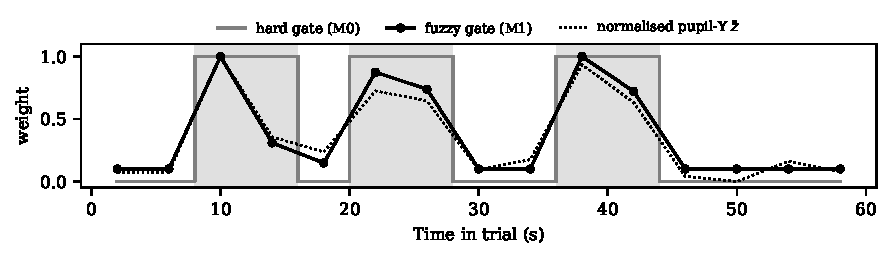
\includegraphics[width=0.85\linewidth]{generated/fig_gate_trace.pdf}
\caption{Hard and fuzzy gate weights on one synthetic trial (SIM-E, subject S01, trial T01) with the G-pupil feature\simnote. Shaded windows overlap a simulated episode.}
\label{fig:trace}
\end{figure}

\subsection{Overall comparison}
Table~\ref{tab:main} reports metrics averaged over bands and seeds for G-pupil. With an informative gating signal, gating of any form helped substantially. Under P1, mean accuracy rose from 35.8\% (A1) to 55.2\% (M0) and 54.9\% (M1) on SIM-H, and from 49.1\% to 66.0\% and 65.7\% on SIM-E. Macro-F1 followed the same pattern (SIM-H 32.8\%, 53.1\%, 52.1\%; SIM-E 45.8\%, 63.9\%, 62.8\%). LOSO gave similar values (SIM-H: 39.9\%, 52.6\%, 54.0\%; SIM-E: 47.4\%, 66.1\%, 65.9\%). The difference between M1 and M0 is at most 1.4~pp in either direction in all four dataset--protocol cells. The linear gate A4 was within 4.4~pp of both. The large standard deviations reflect differences between bands rather than between seeds (Sect.~\ref{sec:bands}).

\begin{table}[t]
\centering\scriptsize
\caption{Trial-level performance with the G-pupil gating feature\simnote{} (\%, mean $\pm$ SD over 5 bands $\times$ 3 seeds). Top: P1 trial-disjoint 5-fold CV; bottom: P2 LOSO}\label{tab:main}
\begin{tabular}{@{}llccccc@{}}
\toprule
Data & Configuration & Accuracy & Bal.\ acc. & Macro P & Macro R & Macro F1\\
\midrule
SIM-H & No gate (A1) & 35.8 $\pm$ 9.2 & 35.8 $\pm$ 9.2 & 39.1 $\pm$ 14.6 & 35.8 $\pm$ 9.2 & 32.8 $\pm$ 9.7\\
 & Hard gate, M0 & 55.2 $\pm$ 25.0 & 55.2 $\pm$ 25.0 & 55.9 $\pm$ 26.4 & 55.2 $\pm$ 25.0 & 53.1 $\pm$ 25.0\\
 & Fuzzy gate, M1 & 54.9 $\pm$ 20.7 & 54.9 $\pm$ 20.7 & 52.4 $\pm$ 20.4 & 54.9 $\pm$ 20.7 & 52.1 $\pm$ 20.6\\
 & Linear soft gate (A4) & 53.2 $\pm$ 18.3 & 53.2 $\pm$ 18.3 & 52.4 $\pm$ 17.3 & 53.2 $\pm$ 18.3 & 50.6 $\pm$ 16.9\\
\midrule
SIM-E & No gate (A1) & 49.1 $\pm$ 8.4 & 49.1 $\pm$ 8.4 & 52.0 $\pm$ 12.6 & 49.1 $\pm$ 8.4 & 45.8 $\pm$ 7.4\\
 & Hard gate, M0 & 66.0 $\pm$ 21.3 & 66.0 $\pm$ 21.3 & 66.3 $\pm$ 24.2 & 66.0 $\pm$ 21.3 & 63.9 $\pm$ 22.7\\
 & Fuzzy gate, M1 & 65.7 $\pm$ 21.1 & 65.7 $\pm$ 21.1 & 65.3 $\pm$ 24.1 & 65.7 $\pm$ 21.1 & 62.8 $\pm$ 22.1\\
 & Linear soft gate (A4) & 64.8 $\pm$ 15.2 & 64.8 $\pm$ 15.2 & 65.0 $\pm$ 20.2 & 64.8 $\pm$ 15.2 & 61.0 $\pm$ 16.0\\
\bottomrule
\end{tabular}
\\[4pt]
\begin{tabular}{@{}llccccc@{}}
\toprule
Data & Configuration & Accuracy & Bal.\ acc. & Macro P & Macro R & Macro F1\\
\midrule
SIM-H & No gate (A1) & 39.9 $\pm$ 12.3 & 39.9 $\pm$ 12.3 & 43.2 $\pm$ 15.5 & 39.9 $\pm$ 12.3 & 36.7 $\pm$ 11.6\\
 & Hard gate, M0 & 52.6 $\pm$ 25.5 & 52.6 $\pm$ 25.5 & 52.4 $\pm$ 25.4 & 52.6 $\pm$ 25.5 & 51.4 $\pm$ 25.6\\
 & Fuzzy gate, M1 & 54.0 $\pm$ 20.5 & 54.0 $\pm$ 20.5 & 52.2 $\pm$ 17.9 & 54.0 $\pm$ 20.5 & 51.2 $\pm$ 19.7\\
 & Linear soft gate (A4) & 57.0 $\pm$ 21.1 & 57.0 $\pm$ 21.1 & 58.4 $\pm$ 23.6 & 57.0 $\pm$ 21.1 & 54.4 $\pm$ 20.7\\
\midrule
SIM-E & No gate (A1) & 47.4 $\pm$ 10.4 & 47.4 $\pm$ 10.4 & 50.4 $\pm$ 11.6 & 47.4 $\pm$ 10.4 & 44.3 $\pm$ 10.0\\
 & Hard gate, M0 & 66.1 $\pm$ 22.4 & 66.1 $\pm$ 22.4 & 65.5 $\pm$ 24.3 & 66.1 $\pm$ 22.4 & 64.1 $\pm$ 23.6\\
 & Fuzzy gate, M1 & 65.9 $\pm$ 18.6 & 65.9 $\pm$ 18.6 & 65.2 $\pm$ 21.9 & 65.9 $\pm$ 18.6 & 63.8 $\pm$ 19.6\\
 & Linear soft gate (A4) & 64.2 $\pm$ 19.3 & 64.2 $\pm$ 19.3 & 64.2 $\pm$ 23.7 & 64.2 $\pm$ 19.3 & 61.8 $\pm$ 20.9\\
\bottomrule
\end{tabular}

\end{table}

Table~\ref{tab:auto} gives the same metrics for G-mRMR. With fixation features as the gating signal, gating had little effect. On SIM-H all configurations lay between 35.8\% and 36.9\% under P1. On SIM-E under P1, M0 was \emph{below} the no-gate reference (44.6\% vs 49.1\%), with M1 at 47.9\%. Under LOSO on SIM-E, M1 (52.3\%) was slightly above M0 (50.6\%) and A1 (47.4\%).

\begin{table}[t]
\centering\scriptsize
\caption{Trial-level performance with the G-mRMR gating feature\simnote{} (\%, mean $\pm$ SD over 5 bands $\times$ 3 seeds). Top: P1; bottom: P2 LOSO}\label{tab:auto}
\begin{tabular}{@{}llccccc@{}}
\toprule
Data & Configuration & Accuracy & Bal.\ acc. & Macro P & Macro R & Macro F1\\
\midrule
SIM-H & No gate (A1) & 35.8 $\pm$ 9.2 & 35.8 $\pm$ 9.2 & 39.1 $\pm$ 14.6 & 35.8 $\pm$ 9.2 & 32.8 $\pm$ 9.7\\
 & Hard gate, M0 & 36.9 $\pm$ 10.2 & 36.9 $\pm$ 10.2 & 40.2 $\pm$ 14.3 & 36.9 $\pm$ 10.2 & 35.5 $\pm$ 10.4\\
 & Fuzzy gate, M1 & 36.9 $\pm$ 10.9 & 36.9 $\pm$ 10.9 & 37.5 $\pm$ 12.9 & 36.9 $\pm$ 10.9 & 35.0 $\pm$ 11.4\\
 & Linear soft gate (A4) & 36.9 $\pm$ 11.9 & 36.9 $\pm$ 11.9 & 36.7 $\pm$ 12.7 & 36.9 $\pm$ 11.9 & 35.1 $\pm$ 12.0\\
\midrule
SIM-E & No gate (A1) & 49.1 $\pm$ 8.4 & 49.1 $\pm$ 8.4 & 52.0 $\pm$ 12.6 & 49.1 $\pm$ 8.4 & 45.8 $\pm$ 7.4\\
 & Hard gate, M0 & 44.6 $\pm$ 12.1 & 44.6 $\pm$ 12.1 & 48.3 $\pm$ 17.3 & 44.6 $\pm$ 12.1 & 43.4 $\pm$ 14.1\\
 & Fuzzy gate, M1 & 47.9 $\pm$ 13.0 & 47.9 $\pm$ 13.0 & 50.7 $\pm$ 16.6 & 47.9 $\pm$ 13.0 & 46.5 $\pm$ 14.2\\
 & Linear soft gate (A4) & 47.8 $\pm$ 11.7 & 47.8 $\pm$ 11.7 & 51.5 $\pm$ 16.5 & 47.8 $\pm$ 11.7 & 46.6 $\pm$ 12.5\\
\bottomrule
\end{tabular}
\\[4pt]
\begin{tabular}{@{}llccccc@{}}
\toprule
Data & Configuration & Accuracy & Bal.\ acc. & Macro P & Macro R & Macro F1\\
\midrule
SIM-H & No gate (A1) & 39.9 $\pm$ 12.3 & 39.9 $\pm$ 12.3 & 43.2 $\pm$ 15.5 & 39.9 $\pm$ 12.3 & 36.7 $\pm$ 11.6\\
 & Hard gate, M0 & 36.4 $\pm$ 9.1 & 36.4 $\pm$ 9.1 & 38.9 $\pm$ 10.6 & 36.4 $\pm$ 9.1 & 36.2 $\pm$ 9.1\\
 & Fuzzy gate, M1 & 38.2 $\pm$ 11.9 & 38.2 $\pm$ 11.9 & 38.5 $\pm$ 12.9 & 38.2 $\pm$ 11.9 & 36.1 $\pm$ 11.8\\
 & Linear soft gate (A4) & 40.2 $\pm$ 11.2 & 40.2 $\pm$ 11.2 & 42.7 $\pm$ 13.9 & 40.2 $\pm$ 11.2 & 37.9 $\pm$ 11.7\\
\midrule
SIM-E & No gate (A1) & 47.4 $\pm$ 10.4 & 47.4 $\pm$ 10.4 & 50.4 $\pm$ 11.6 & 47.4 $\pm$ 10.4 & 44.3 $\pm$ 10.0\\
 & Hard gate, M0 & 50.6 $\pm$ 15.9 & 50.6 $\pm$ 15.9 & 51.9 $\pm$ 20.7 & 50.6 $\pm$ 15.9 & 49.1 $\pm$ 17.4\\
 & Fuzzy gate, M1 & 52.3 $\pm$ 16.2 & 52.3 $\pm$ 16.2 & 54.1 $\pm$ 18.2 & 52.3 $\pm$ 16.2 & 50.8 $\pm$ 16.6\\
 & Linear soft gate (A4) & 50.9 $\pm$ 16.8 & 50.9 $\pm$ 16.8 & 54.3 $\pm$ 18.6 & 50.9 $\pm$ 16.8 & 49.0 $\pm$ 17.8\\
\bottomrule
\end{tabular}

\end{table}

\subsection{Frequency-band analysis}
\label{sec:bands}
Table~\ref{tab:bands} and Fig.~\ref{fig:bands} break the G-pupil results down by band. As designed into the simulation, alpha, beta and gamma carry most class information, and delta and theta stay near chance. In the informative bands the gates trade places. Under P1, M1 was better than M0 in alpha (72.2\% vs 70.6\% on SIM-H; 77.2\% vs 73.9\% on SIM-E) and theta, whereas M0 was better in beta and gamma (SIM-H gamma 78.9\% vs 71.1\%; SIM-E gamma 91.7\% vs 90.6\%). The highest accuracy in the study, 91.7\% (SIM-E, gamma, M0), is far above the no-gate value for the same band (48.3\%), which shows how much the class signal is diluted by non-episode windows when no gate is applied.

\begin{table}[t]
\centering\scriptsize
\caption{Trial-level accuracy per band with G-pupil\simnote{} (\%, mean $\pm$ SD over 3 seeds; best per band and dataset in bold). Top: P1; bottom: P2 LOSO}\label{tab:bands}
\resizebox{\linewidth}{!}{\begin{tabular}{@{}llccccc@{}}
\toprule
Data & Configuration & Delta & Theta & Alpha & Beta & Gamma\\
\midrule
SIM-H & No gate (A1) & 27.2 $\pm$ 3.4 & 27.8 $\pm$ 0.8 & 38.9 $\pm$ 1.6 & 51.1 $\pm$ 3.4 & 33.9 $\pm$ 2.8\\
 & Hard gate, M0 & 24.4 $\pm$ 3.1 & 25.6 $\pm$ 2.8 & 70.6 $\pm$ 4.2 & \textbf{76.7 $\pm$ 0.0} & \textbf{78.9 $\pm$ 2.8}\\
 & Fuzzy gate, M1 & 25.0 $\pm$ 1.4 & \textbf{35.6 $\pm$ 4.4} & \textbf{72.2 $\pm$ 6.4} & 70.6 $\pm$ 0.8 & 71.1 $\pm$ 2.8\\
 & Linear soft gate (A4) & \textbf{27.8 $\pm$ 3.9} & 35.0 $\pm$ 2.4 & 63.3 $\pm$ 1.4 & 69.4 $\pm$ 2.1 & 70.6 $\pm$ 0.8\\
\midrule
SIM-E & No gate (A1) & 40.6 $\pm$ 0.8 & 42.2 $\pm$ 6.8 & 53.9 $\pm$ 3.4 & 60.6 $\pm$ 3.1 & 48.3 $\pm$ 2.4\\
 & Hard gate, M0 & 36.1 $\pm$ 4.8 & 47.2 $\pm$ 5.7 & 73.9 $\pm$ 0.8 & \textbf{81.1 $\pm$ 0.8} & \textbf{91.7 $\pm$ 4.7}\\
 & Fuzzy gate, M1 & 33.3 $\pm$ 1.4 & 49.4 $\pm$ 1.6 & \textbf{77.2 $\pm$ 0.8} & 77.8 $\pm$ 2.1 & 90.6 $\pm$ 2.8\\
 & Linear soft gate (A4) & \textbf{42.8 $\pm$ 2.8} & \textbf{51.7 $\pm$ 2.4} & 70.6 $\pm$ 2.1 & 77.8 $\pm$ 0.8 & 81.1 $\pm$ 3.4\\
\bottomrule
\end{tabular}
}\\[4pt]
\resizebox{\linewidth}{!}{\begin{tabular}{@{}llccccc@{}}
\toprule
Data & Configuration & Delta & Theta & Alpha & Beta & Gamma\\
\midrule
SIM-H & No gate (A1) & 25.0 $\pm$ 2.4 & 25.6 $\pm$ 2.1 & 48.3 $\pm$ 2.7 & 51.7 $\pm$ 4.9 & 48.9 $\pm$ 0.8\\
 & Hard gate, M0 & 22.8 $\pm$ 4.8 & 20.6 $\pm$ 1.6 & 69.4 $\pm$ 0.8 & \textbf{73.9 $\pm$ 1.6} & \textbf{76.1 $\pm$ 4.8}\\
 & Fuzzy gate, M1 & 28.9 $\pm$ 4.2 & 29.4 $\pm$ 1.6 & 67.2 $\pm$ 1.6 & \textbf{73.9 $\pm$ 1.6} & 70.6 $\pm$ 0.8\\
 & Linear soft gate (A4) & \textbf{30.6 $\pm$ 1.6} & \textbf{32.2 $\pm$ 3.1} & \textbf{76.7 $\pm$ 1.4} & 71.7 $\pm$ 2.4 & 73.9 $\pm$ 2.1\\
\midrule
SIM-E & No gate (A1) & 35.0 $\pm$ 3.6 & 38.3 $\pm$ 5.9 & 50.6 $\pm$ 4.4 & 60.0 $\pm$ 1.4 & 53.3 $\pm$ 5.9\\
 & Hard gate, M0 & 30.0 $\pm$ 1.4 & \textbf{52.8 $\pm$ 3.4} & \textbf{73.3 $\pm$ 3.6} & 82.2 $\pm$ 2.1 & \textbf{92.2 $\pm$ 2.1}\\
 & Fuzzy gate, M1 & 38.9 $\pm$ 3.4 & 51.7 $\pm$ 4.7 & 68.3 $\pm$ 1.4 & \textbf{83.9 $\pm$ 2.1} & 86.7 $\pm$ 2.4\\
 & Linear soft gate (A4) & \textbf{42.8 $\pm$ 0.8} & 41.7 $\pm$ 2.7 & 66.7 $\pm$ 4.1 & 83.3 $\pm$ 1.4 & 86.7 $\pm$ 1.4\\
\bottomrule
\end{tabular}
}
\end{table}

\begin{figure}[t]
\centering
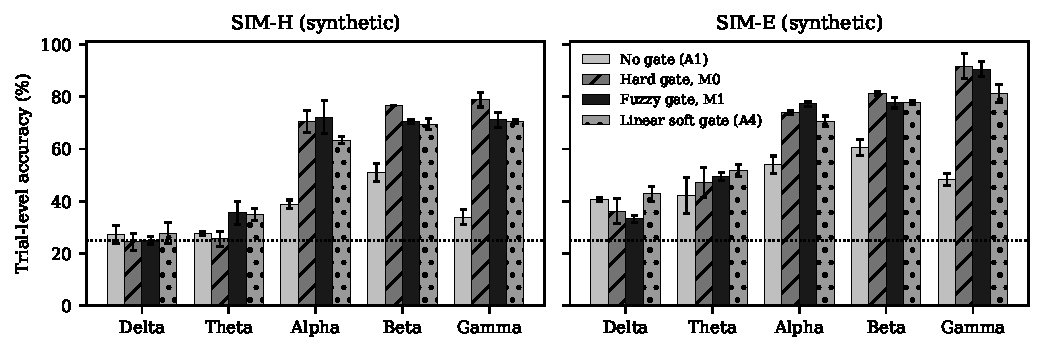
\includegraphics[width=\linewidth]{generated/fig_bands.pdf}
\caption{Trial-level accuracy per band, G-pupil, protocol P1\simnote{} (mean $\pm$ SD over 3 seeds). The dotted line marks chance (25\%).}
\label{fig:bands}
\end{figure}

\subsection{Class-wise behaviour}
Figure~\ref{fig:cm} shows the confusion matrices of M0 and M1 for the best band of SIM-E (gamma, P1, pooled over three seeds, 45 trials per class). The two gates make almost the same errors. Sad, happy and neutral trials are recognised almost perfectly, and fear is the weak class: 31 of 45 fear trials are correct under M0 and 29 under M1, with most errors assigned to neutral (12 and 13 trials). This is consistent with the generator, in which the bursty broadband fear component is the least stationary within a window.

\begin{figure}[t]
\centering
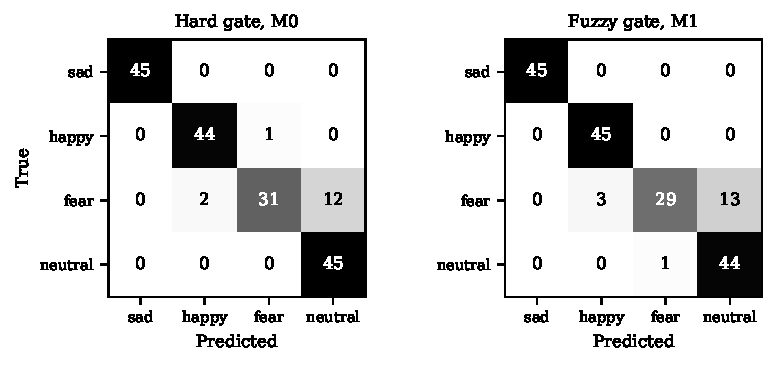
\includegraphics[width=0.72\linewidth]{generated/fig_confusion.pdf}
\caption{Trial-level confusion matrices for M0 and M1, SIM-E, gamma band, G-pupil, P1, pooled over three seeds\simnote.}
\label{fig:cm}
\end{figure}

\subsection{Statistical comparison}
Table~\ref{tab:stats} reports the paired tests. With G-pupil, M1 differed from M0 by a median of 0 to $-1.7$~pp, and no difference approached significance ($p=0.407$--$0.916$). M1 did not differ significantly from the linear gate either ($p\geq0.093$). M1 was, however, clearly better than no gating ($p\leq0.005$; 11--15 wins out of 15 pairs; median gains 16.7--21.7~pp). The exact McNemar tests for the best bands agree: on SIM-H alpha, 30 trials were correct only under M1 and 27 only under M0 ($p=0.79$); on SIM-E gamma the counts were 12 and 14 ($p=0.85$). With G-mRMR, two of the twelve M1 comparisons reached $p<0.05$ (M1 vs M0, LOSO, SIM-E, median $+1.7$~pp, $p=0.049$; and M1 vs A1 in the same cell, $p=0.041$). Given the number of tests performed, these isolated results do not survive correction for multiple comparisons and are not taken as evidence of an advantage.

\begin{table}[t]
\centering\scriptsize
\caption{Paired Wilcoxon signed-rank tests of M1 against other gates over 15 (seed, band) pairs\simnote. $\Delta$acc: M1 minus comparator. Uncorrected $p$-values}\label{tab:stats}
\resizebox{\linewidth}{!}{\begin{tabular}{@{}lllcccc@{}}
\toprule
Gate feature & Protocol & Data & Comparison & Median $\Delta$acc (pp) & W / wins--ties--losses & $p$\\
\midrule
pupil-Y & trial-disjoint 5-fold & SIM-H & M1 vs Hard gate & +0.0 & 41 / 6--2--7 & 0.752\\
pupil-Y & trial-disjoint 5-fold & SIM-H & M1 vs Linear soft gate & +0.0 & 34 / 7--2--6 & 0.442\\
pupil-Y & trial-disjoint 5-fold & SIM-H & M1 vs No gate & +18.3 & 4 / 13--1--1 & 0.002\\
pupil-Y & trial-disjoint 5-fold & SIM-E & M1 vs Hard gate & -1.7 & 58 / 7--0--8 & 0.886\\
pupil-Y & trial-disjoint 5-fold & SIM-E & M1 vs Linear soft gate & +0.0 & 44 / 7--1--7 & 0.572\\
pupil-Y & trial-disjoint 5-fold & SIM-E & M1 vs No gate & +20.0 & 10 / 11--0--4 & 0.005\\
\midrule
pupil-Y & LOSO & SIM-H & M1 vs Hard gate & +0.0 & 16 / 5--6--4 & 0.407\\
pupil-Y & LOSO & SIM-H & M1 vs Linear soft gate & -1.7 & 30 / 5--0--10 & 0.093\\
pupil-Y & LOSO & SIM-H & M1 vs No gate & +16.7 & 0 / 14--1--0 & 0.001\\
pupil-Y & LOSO & SIM-E & M1 vs Hard gate & +0.0 & 44 / 7--2--6 & 0.916\\
pupil-Y & LOSO & SIM-E & M1 vs Linear soft gate & +1.7 & 31 / 8--2--5 & 0.308\\
pupil-Y & LOSO & SIM-E & M1 vs No gate & +21.7 & 0 / 15--0--0 & 0.001\\
\midrule
mRMR & trial-disjoint 5-fold & SIM-H & M1 vs Hard gate & +0.0 & 45 / 7--2--6 & 0.972\\
mRMR & trial-disjoint 5-fold & SIM-H & M1 vs Linear soft gate & +0.0 & 49 / 7--1--7 & 0.826\\
mRMR & trial-disjoint 5-fold & SIM-H & M1 vs No gate & +1.7 & 50 / 8--0--7 & 0.585\\
mRMR & trial-disjoint 5-fold & SIM-E & M1 vs Hard gate & +3.3 & 27 / 9--1--5 & 0.109\\
mRMR & trial-disjoint 5-fold & SIM-E & M1 vs Linear soft gate & +0.0 & 32 / 5--4--6 & 0.929\\
mRMR & trial-disjoint 5-fold & SIM-E & M1 vs No gate & +1.7 & 53 / 8--0--7 & 0.691\\
\midrule
mRMR & LOSO & SIM-H & M1 vs Hard gate & +1.7 & 37 / 8--1--6 & 0.328\\
mRMR & LOSO & SIM-H & M1 vs Linear soft gate & +0.0 & 18 / 4--4--7 & 0.180\\
mRMR & LOSO & SIM-H & M1 vs No gate & -1.7 & 24 / 4--2--9 & 0.140\\
mRMR & LOSO & SIM-E & M1 vs Hard gate & +1.7 & 26 / 10--0--5 & 0.049\\
mRMR & LOSO & SIM-E & M1 vs Linear soft gate & +1.7 & 28 / 9--1--5 & 0.130\\
mRMR & LOSO & SIM-E & M1 vs No gate & +8.3 & 24 / 11--0--4 & 0.041\\
\bottomrule
\end{tabular}
}
\end{table}

\subsection{Robustness to gate-signal noise}
The main argument for fuzzy gating is tolerance of an uncertain eye signal. Table~\ref{tab:noise} and Fig.~\ref{fig:noise} test this directly. As noise increased from $\kappa=0$ to $\kappa=2$, the AUC of the pupil feature for detecting episodes fell from about 0.99 to 0.72--0.73, and all gated configurations lost accuracy (M0: 55.2\% to 43.8\% on SIM-H and 66.0\% to 55.1\% on SIM-E). The fuzzy gate did \emph{not} degrade more gracefully. Its mean deficit relative to M0 was between $-1.1$ and $-3.4$~pp at every non-zero noise level, although none of these differences was significant ($p\geq0.19$). At every noise level all gates remained above the no-gate reference. The hypothesis that fuzzy gating confers robustness to gate noise is therefore not supported by this simulation.

\begin{table}[t]
\centering\scriptsize
\caption{Mean trial accuracy (\%) under gate-signal noise\simnote{} (G-pupil, P1, mean over 5 bands $\times$ 3 seeds). Gate AUC: episode-detection AUC of the noisy pupil feature. $p$: Wilcoxon, M1 vs M0}\label{tab:noise}
\begin{tabular}{@{}lcccccccc@{}}
\toprule
Data & Noise $\kappa$ & Gate AUC & No gate & M0 hard & M1 fuzzy & A4 linear & $\Delta$(M1$-$M0) & $p$\\
\midrule
SIM-H & 0 & 0.987 & 35.8 & 55.2 & 54.9 & 53.2 & -0.3 & 0.752\\
 & 0.5 & 0.943 & 35.8 & 53.1 & 51.7 & 52.0 & -1.4 & 0.299\\
 & 1 & 0.852 & 35.8 & 50.0 & 47.4 & 47.4 & -2.6 & 0.191\\
 & 2 & 0.721 & 35.8 & 43.8 & 41.7 & 44.3 & -2.1 & 0.310\\
\midrule
SIM-E & 0 & 0.985 & 49.1 & 66.0 & 65.7 & 64.8 & -0.3 & 0.886\\
 & 0.5 & 0.943 & 49.1 & 65.0 & 63.9 & 61.7 & -1.1 & 0.506\\
 & 1 & 0.855 & 49.1 & 62.7 & 59.8 & 60.4 & -2.9 & 0.258\\
 & 2 & 0.729 & 49.1 & 55.1 & 51.7 & 53.8 & -3.4 & 0.363\\
\bottomrule
\end{tabular}

\end{table}

\begin{figure}[t]
\centering
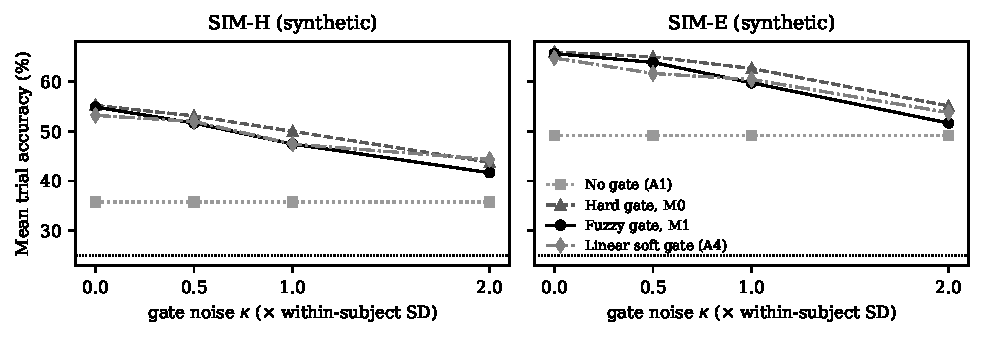
\includegraphics[width=0.95\linewidth]{generated/fig_noise.pdf}
\caption{Mean trial accuracy as a function of gate-signal noise $\kappa$, G-pupil, P1\simnote.}
\label{fig:noise}
\end{figure}

\subsection{Computational cost}
Table~\ref{tab:cost} reports the effective share of training windows (sum of weights divided by the number of windows) and the mean wall-clock time per band and run (all folds). Because the GA dominates the run time and stops adaptively, all gates cost about the same, 10.9--11.6~s per band. The baseline's argument that gating saves computation by discarding windows \cite{FarhadiSedehi2024a} applies to feature extraction on real-time hardware, which is identical here because entropies were precomputed for all windows. In such a setting the fuzzy gate would forgo that saving, since every window must be processed.

\begin{table}[t]
\centering\small
\caption{Computational cost\simnote{} (mean over all runs)}\label{tab:cost}
\begin{tabular}{@{}lcc@{}}
\toprule
Configuration & Effective training windows (\%) & Time per band, all folds (s)\\
\midrule
No gate (A1) & 100.0 & 11.6\\
Hard gate, M0 & 41.8 & 11.0\\
Fuzzy gate, M1 & 45.7 & 11.2\\
Linear soft gate (A4) & 44.3 & 10.9\\
\bottomrule
\end{tabular}

\end{table}

\subsection{Relation to the team's earlier window-level runs}
Before this study, the baseline pipeline (M0 only) had been run on the same synthetic datasets with the original protocol, in which 4-s windows are pooled and randomly split into five folds and accuracy is measured per window. Those runs are reported in Table~\ref{tab:prev} for completeness. They are window-level accuracies on the retained windows, not trial-level accuracies, and are therefore not directly comparable with Tables~\ref{tab:main}--\ref{tab:noise}. Two observations agree with the present study: the run that used the fixation-duration gate selected by mRMR reached at most 47.8\% (SIM-H) and 56.7\% (SIM-E), whereas the run with the pupil gate reached 75.0--75.8\% in beta and gamma on SIM-E. On these synthetic data, where windows are generated independently given the episode mask, the trial-grouped protocol gave values similar to the pooled protocol (e.g.\ SIM-H beta 45.8\% vs 47.8\%). This similarity is not expected to hold for real EEG, where neighbouring windows are strongly correlated \cite{Li2021}.

\begin{table}[t]
\centering\scriptsize
\caption{Earlier baseline (M0) runs on the synthetic data with the original window-level protocol\simnote{} (window accuracy on retained windows, \%, mean $\pm$ SD over 5 folds, 3 fuzzy levels)}\label{tab:prev}
\resizebox{\linewidth}{!}{\begin{tabular}{@{}llccccc@{}}
\toprule
Run & Gate feature / protocol & Delta & Theta & Alpha & Beta & Gamma\\
\midrule
SIM-H & mRMR (\texttt{fix\_dur\_mean}) / window 5-fold & 20.8 $\pm$ 2.3 & 23.6 $\pm$ 4.2 & 43.3 $\pm$ 2.7 & 47.8 $\pm$ 4.8 & 47.2 $\pm$ 3.4\\
SIM-H & mRMR (\texttt{fix\_dur\_mean}) / trial-grouped & 26.1 $\pm$ 4.2 & 25.0 $\pm$ 2.8 & 42.5 $\pm$ 4.8 & 45.8 $\pm$ 7.1 & 46.7 $\pm$ 3.4\\
SIM-E & mRMR (\texttt{fix\_dur\_mean}) / window 5-fold & 24.2 $\pm$ 5.1 & 30.8 $\pm$ 5.9 & 50.8 $\pm$ 2.6 & 56.7 $\pm$ 3.2 & 54.2 $\pm$ 4.7\\
SIM-E & \texttt{pupil\_y\_mean} / window 5-fold & 33.6 $\pm$ 4.4 & 35.3 $\pm$ 5.9 & 59.7 $\pm$ 3.2 & 75.0 $\pm$ 6.8 & 75.8 $\pm$ 2.4\\
\bottomrule
\end{tabular}
}
\end{table}

\subsection{Discussion}
Three findings stand out. First, \emph{the gating signal matters far more than the gating function}. With a signal that tracks the informative windows, any of the three gates raised mean accuracy by 13--19~pp over no gating; with a class-discriminative but episode-blind signal, none helped reliably. This exposes a weakness of the original procedure, which selects the gate feature by its mutual information with the class label. Such a criterion rewards features that differ \emph{between} classes, whereas a gate needs a feature that differs \emph{within} a trial between affective and non-affective moments. In our simulation the two criteria point to different features. In real data, label-driven selection can also pick up session or stimulus confounds.

Second, \emph{fuzzy and hard gating were statistically indistinguishable}, and the fuzzy gate was not better than a plain linear soft gate. With one input and a Ruspini partition, the fuzzy gate is a piecewise-linear soft threshold, so this equivalence is unsurprising in hindsight. The data show no benefit from the fuzzy formulation itself beyond what its softness provides.

Third, \emph{softness did not buy robustness}. The fuzzy gate keeps every window with weight at least $r_L$ and gives Medium-range windows substantial weight, which lowers its weighted precision (79\% vs 90--93\% for the hard gate). When class information is confined to the episodes, as in this simulation, the extra non-episode mass dilutes the training data and the trial vote. When gate noise rises, the soft gate does not recover this loss. A softer gate would be expected to help mainly when the gating signal is weakly informative and the hard gate's ranking within a trial becomes unreliable. Even at $\kappa=2$ (AUC 0.72), that point had not been reached. The design parameters ($r_L=0.1$, the width of the Medium set) were fixed a priori, and a sharper partition or a learned partition might change this balance. That is a question for future work, not a finding of this study.

The interpretability argument for fuzzy gating is unaffected by these results. The gate can be stated as three linguistic rules, and a reviewer can read off how much each window contributed. The value of that transparency has to be weighed against the absence of an accuracy advantage.

% =====================================================================
\section{Limitations}
\label{sec:limits}
(i) \emph{All results are on synthetic data.} The generator encodes the assumptions that motivate gating, namely intermittent affective information and pupil dilation co-occurring with it. The results show how the gates behave if these assumptions hold, not whether they hold in real recordings or what accuracy would be obtained on real EEG. (ii) The synthetic data are small (5 subjects, 60 trials), so differences of a few percentage points cannot be resolved. With 15 paired observations per test, the study can detect only moderate effects. (iii) Synthetic windows are conditionally independent given the episode mask, so the leakage that pooled window-level cross-validation causes on real EEG is not reproduced. (iv) The hard-gate threshold rule (within-trial 60th percentile) is our operationalisation of an under-specified description \cite{FarhadiSedehi2024a}, and the fuzzy-gate parameters were not tuned. Other choices could shift the comparison. (v) The pupil signal in the simulation contains no luminance or gaze-position confounds \cite{Mathot2018,Raiturkar2016}, which are major sources of uncertainty in real recordings. (vi) The S-FIS uses only three EEG inputs per band, as in the original method.

% =====================================================================
\section{Conclusion and future work}
\label{sec:conclusion}
This paper compared hard and fuzzy eye-tracking gating of EEG windows within a Sugeno fuzzy rule-mining emotion recognizer. All other components were held fixed, and the evaluation was a controlled simulation in which the affectively relevant windows are known. The fuzzy gate maps Low/Medium/High memberships of the normalised eye-tracking feature to continuous window weights that enter feature selection, rule mining, GA fitness and trial-level aggregation, and it contains the hard gate as a limiting case. On two synthetic datasets, under trial- and subject-disjoint cross-validation, gating with an informative pupil signal improved trial accuracy over no gating by median paired gains of 16.7--21.7 percentage points. Fuzzy and hard gating, however, were statistically indistinguishable. The fuzzy gate was not better than a linear soft gate and not more robust to gate-signal noise. Selecting the gate feature by its relevance to the class label, as in the original method, chose fixation features that did not locate the informative windows. In this setting, how well the gating signal identifies the relevant windows matters far more than the form of the gate.

Future work will (1) evaluate the gates on real simultaneous EEG and eye-tracking recordings such as SEED-IV \cite{Zheng2019}, MAHNOB-HCI \cite{Soleymani2012db} or ZuCo \cite{Hollenstein2018}, under subject-disjoint protocols; (2) select gating features by within-trial relevance criteria rather than class relevance; (3) correct pupil signals for luminance before gating \cite{Raiturkar2016}; (4) study multi-input fuzzy gates and gate parameters learned under nested cross-validation \cite{Jang1993}; and (5) extend the simulation with temporally correlated windows and realistic ocular confounds.

% =====================================================================
\section*{Declarations}
\noindent\textbf{Funding} \pending{to be completed by the authors}\\
\textbf{Conflict of interest} \pending{to be completed by the authors}\\
\textbf{Data availability} No real human data were used. The synthetic datasets can be regenerated exactly with \texttt{python -m gfer.demo --out data/demo --seed 0} (SIM-H) and \texttt{python -m gfer.demo --out data/demo\_easy --seed 1 --signal-strength 3} (SIM-E).\\
\textbf{Code availability} All code, raw results and the scripts that generate every table and figure (\texttt{gfer/compare.py}, \texttt{gfer/analyze\_sim.py}, \texttt{gfer/analyze\_noise.py}) are available at \pending{repository URL}.\\
\textbf{Author contributions} \pending{to be completed by the authors}

% =====================================================================
\small
\begin{thebibliography}{99}

\bibitem{Alarcao2019} Alarc\~ao SM, Fonseca MJ (2019) Emotions recognition using EEG signals: a survey. IEEE Trans Affect Comput 10(3):374--393. \url{https://doi.org/10.1109/TAFFC.2017.2714671}

\bibitem{Arevalo2020} Arevalo J, Solorio T, Montes-y-G\'omez M, Gonz\'alez FA (2020) Gated multimodal networks. Neural Comput Appl 32(14):10209--10228. \url{https://doi.org/10.1007/s00521-019-04559-1}

\bibitem{Bandt2002} Bandt C, Pompe B (2002) Permutation entropy: a natural complexity measure for time series. Phys Rev Lett 88(17):174102. \url{https://doi.org/10.1103/PhysRevLett.88.174102}

\bibitem{Bradley2008} Bradley MM, Miccoli L, Escrig MA, Lang PJ (2008) The pupil as a measure of emotional arousal and autonomic activation. Psychophysiology 45(4):602--607. \url{https://doi.org/10.1111/j.1469-8986.2008.00654.x}

\bibitem{ChoKim1995} Cho SB, Kim JH (1995) Combining multiple neural networks by fuzzy integral for robust classification. IEEE Trans Syst Man Cybern 25(2):380--384. \url{https://doi.org/10.1109/21.364825}

\bibitem{Demsar2006} Dem\v{s}ar J (2006) Statistical comparisons of classifiers over multiple data sets. J Mach Learn Res 7:1--30

\bibitem{Duan2013} Duan RN, Zhu JY, Lu BL (2013) Differential entropy feature for EEG-based emotion classification. In: 6th Int IEEE/EMBS Conf Neural Engineering (NER), pp 81--84. \url{https://doi.org/10.1109/NER.2013.6695876}

\bibitem{FarhadiSedehi2024a} Farhadi Sedehi J, Jafarnia Dabanloo N, Maghooli K, Sheikhani A (2024) Recognition of emotional categories using mined fuzzy rules from electroencephalogram signals with gated eye track data approach. IEEE Access 12:118122--118140. \url{https://doi.org/10.1109/ACCESS.2024.3430934}

\bibitem{FarhadiSedehi2024b} Farhadi Sedehi J, Jafarnia Dabanloo N, Maghooli K, Sheikhani A (2024) Multimodal insights into Granger causality connectivity: integrating physiological signals and gated eye-tracking data for emotion recognition using convolutional neural network. Heliyon 10(16):e36411. \url{https://doi.org/10.1016/j.heliyon.2024.e36411}

\bibitem{Fu2023} Fu B, Gu C, Fu M, Xia Y, Liu Y (2023) A novel feature fusion network for multimodal emotion recognition from EEG and eye movement signals. Front Neurosci 17:1234162. \url{https://doi.org/10.3389/fnins.2023.1234162}

\bibitem{Hollenstein2018} Hollenstein N, Rotsztejn J, Troendle M, Pedroni A, Zhang C, Langer N (2018) ZuCo, a simultaneous EEG and eye-tracking resource for natural sentence reading. Sci Data 5:180291. \url{https://doi.org/10.1038/sdata.2018.291}

\bibitem{Holmqvist2012} Holmqvist K, Nystr\"om M, Mulvey F (2012) Eye tracker data quality: what it is and how to measure it. In: Proc Symp Eye Tracking Research and Applications (ETRA), pp 45--52. \url{https://doi.org/10.1145/2168556.2168563}

\bibitem{Jacobs1991} Jacobs RA, Jordan MI, Nowlan SJ, Hinton GE (1991) Adaptive mixtures of local experts. Neural Comput 3(1):79--87. \url{https://doi.org/10.1162/neco.1991.3.1.79}

\bibitem{Jang1993} Jang JSR (1993) ANFIS: adaptive-network-based fuzzy inference system. IEEE Trans Syst Man Cybern 23(3):665--685. \url{https://doi.org/10.1109/21.256541}

\bibitem{Jenke2014} Jenke R, Peer A, Buss M (2014) Feature extraction and selection for emotion recognition from EEG. IEEE Trans Affect Comput 5(3):327--339. \url{https://doi.org/10.1109/TAFFC.2014.2339834}

\bibitem{Kaya2024} Kaya \"U, Akay D, \c{S}eng\"ul Ayan S (2024) EEG-based emotion recognition in neuromarketing using fuzzy linguistic summarization. IEEE Trans Fuzzy Syst 32(8):4248--4259. \url{https://doi.org/10.1109/TFUZZ.2024.3392495}

\bibitem{Khan2025} Khan NN, Sweet T, Harvey CA, Knapp C, Krusienski DJ, Thompson DE (2025) The role of review process failures in affective state estimation: an empirical investigation of DEAP dataset. arXiv:2508.02417 (preprint)

\bibitem{Kittler1998} Kittler J, Hatef M, Duin RPW, Matas J (1998) On combining classifiers. IEEE Trans Pattern Anal Mach Intell 20(3):226--239. \url{https://doi.org/10.1109/34.667881}

\bibitem{Koelstra2012} Koelstra S, M\"uhl C, Soleymani M, Lee JS, Yazdani A, Ebrahimi T, Pun T, Nijholt A, Patras I (2012) DEAP: a database for emotion analysis using physiological signals. IEEE Trans Affect Comput 3(1):18--31. \url{https://doi.org/10.1109/T-AFFC.2011.15}

\bibitem{Kret2019} Kret ME, Sjak-Shie EE (2019) Preprocessing pupil size data: guidelines and code. Behav Res Methods 51(3):1336--1342. \url{https://doi.org/10.3758/s13428-018-1075-y}

\bibitem{Kukhilava2025} Kukhilava N, Tsmindashvili T, Kalandadze R, et al (2025) Evaluation in EEG emotion recognition: state-of-the-art review and unified framework. arXiv:2505.18175 (preprint)

\bibitem{Li2021} Li R, Johansen JS, Ahmed H, Ilyevsky TV, Wilbur RB, Bharadwaj HM, Siskind JM (2021) The perils and pitfalls of block design for EEG classification experiments. IEEE Trans Pattern Anal Mach Intell 43(1):316--333. \url{https://doi.org/10.1109/TPAMI.2020.2973153}

\bibitem{Lim2020} Lim JZ, Mountstephens J, Teo J (2020) Emotion recognition using eye-tracking: taxonomy, review and current challenges. Sensors 20(8):2384. \url{https://doi.org/10.3390/s20082384}

\bibitem{LinWang2002} Lin CF, Wang SD (2002) Fuzzy support vector machines. IEEE Trans Neural Netw 13(2):464--471. \url{https://doi.org/10.1109/72.991432}

\bibitem{Liu2022} Liu W, Qiu JL, Zheng WL, Lu BL (2022) Comparing recognition performance and robustness of multimodal deep learning models for multimodal emotion recognition. IEEE Trans Cogn Dev Syst 14(2):715--729. \url{https://doi.org/10.1109/TCDS.2021.3071170}

\bibitem{Lu2015} Lu Y, Zheng WL, Li B, Lu BL (2015) Combining eye movements and EEG to enhance emotion recognition. In: Proc 24th Int Joint Conf Artificial Intelligence (IJCAI), pp 1170--1175

\bibitem{Mallat1989} Mallat SG (1989) A theory for multiresolution signal decomposition: the wavelet representation. IEEE Trans Pattern Anal Mach Intell 11(7):674--693. \url{https://doi.org/10.1109/34.192463}

\bibitem{Mathot2018} Math\^ot S (2018) Pupillometry: psychology, physiology, and function. J Cogn 1(1):16. \url{https://doi.org/10.5334/joc.18}

\bibitem{Matiko2014} Matiko JW, Beeby SP, Tudor J (2014) Fuzzy logic based emotion classification. In: Proc IEEE Int Conf Acoustics, Speech and Signal Processing (ICASSP), pp 4389--4393. \url{https://doi.org/10.1109/ICASSP.2014.6854431}

\bibitem{McNemar1947} McNemar Q (1947) Note on the sampling error of the difference between correlated proportions or percentages. Psychometrika 12(2):153--157. \url{https://doi.org/10.1007/BF02295996}

\bibitem{Murugappan2010} Murugappan M, Ramachandran N, Sazali Y (2010) Classification of human emotion from EEG using discrete wavelet transform. J Biomed Sci Eng 3(4):390--396. \url{https://doi.org/10.4236/jbise.2010.34054}

\bibitem{Nandakumar2008} Nandakumar K, Chen Y, Dass SC, Jain AK (2008) Likelihood ratio-based biometric score fusion. IEEE Trans Pattern Anal Mach Intell 30(2):342--347. \url{https://doi.org/10.1109/TPAMI.2007.70796}

\bibitem{Partala2003} Partala T, Surakka V (2003) Pupil size variation as an indication of affective processing. Int J Hum-Comput Stud 59(1--2):185--198. \url{https://doi.org/10.1016/S1071-5819(03)00017-X}

\bibitem{Peng2005} Peng H, Long F, Ding C (2005) Feature selection based on mutual information criteria of max-dependency, max-relevance, and min-redundancy. IEEE Trans Pattern Anal Mach Intell 27(8):1226--1238. \url{https://doi.org/10.1109/TPAMI.2005.159}

\bibitem{Raiturkar2016} Raiturkar P, Kleinsmith A, Keil A, Banerjee A, Jain E (2016) Decoupling light reflex from pupillary dilation to measure emotional arousal in videos. In: Proc ACM Symp Applied Perception (SAP), pp 89--96. \url{https://doi.org/10.1145/2931002.2931009}

\bibitem{Richman2000} Richman JS, Moorman JR (2000) Physiological time-series analysis using approximate entropy and sample entropy. Am J Physiol Heart Circ Physiol 278(6):H2039--H2049. \url{https://doi.org/10.1152/ajpheart.2000.278.6.H2039}

\bibitem{Rohila2019} Rohila A, Sharma A (2019) Phase entropy: a new complexity measure for heart rate variability. Physiol Meas 40(10):105006. \url{https://doi.org/10.1088/1361-6579/ab499e}

\bibitem{Soleymani2012db} Soleymani M, Lichtenauer J, Pun T, Pantic M (2012) A multimodal database for affect recognition and implicit tagging. IEEE Trans Affect Comput 3(1):42--55. \url{https://doi.org/10.1109/T-AFFC.2011.25}

\bibitem{Soleymani2012mm} Soleymani M, Pantic M, Pun T (2012) Multimodal emotion recognition in response to videos. IEEE Trans Affect Comput 3(2):211--223. \url{https://doi.org/10.1109/T-AFFC.2011.37}

\bibitem{TakagiSugeno1985} Takagi T, Sugeno M (1985) Fuzzy identification of systems and its applications to modeling and control. IEEE Trans Syst Man Cybern SMC-15(1):116--132. \url{https://doi.org/10.1109/TSMC.1985.6313399}

\bibitem{WangMendel1992} Wang LX, Mendel JM (1992) Generating fuzzy rules by learning from examples. IEEE Trans Syst Man Cybern 22(6):1414--1427. \url{https://doi.org/10.1109/21.199466}

\bibitem{Zadeh1965} Zadeh LA (1965) Fuzzy sets. Inf Control 8(3):338--353. \url{https://doi.org/10.1016/S0019-9958(65)90241-X}

\bibitem{Zebrowski2000} \.Zebrowski JJ, Pop\l awska W, Baranowski R, Buchner T (2000) Symbolic dynamics and complexity in a physiological time series. Chaos Solitons Fractals 11(7):1061--1075. \url{https://doi.org/10.1016/S0960-0779(99)00004-1}

\bibitem{ZhengDong2014} Zheng WL, Dong BN, Lu BL (2014) Multimodal emotion recognition using EEG and eye tracking data. In: Proc 36th Annu Int Conf IEEE Eng Med Biol Soc (EMBC), pp 5040--5043. \url{https://doi.org/10.1109/EMBC.2014.6944757}

\bibitem{Zheng2019} Zheng WL, Liu W, Lu Y, Lu BL, Cichocki A (2019) EmotionMeter: a multimodal framework for recognizing human emotions. IEEE Trans Cybern 49(3):1110--1122. \url{https://doi.org/10.1109/TCYB.2018.2797176}

\bibitem{ZhengLu2015} Zheng WL, Lu BL (2015) Investigating critical frequency bands and channels for EEG-based emotion recognition with deep neural networks. IEEE Trans Auton Ment Dev 7(3):162--175. \url{https://doi.org/10.1109/TAMD.2015.2431497}

\end{thebibliography}
\end{document}
